\chapter{Statistisches Testen}
\section{Die Logik des Testes}
Die Analogie zum Beweis durch Widerspruch kann hilfreich sein, hier ein Beispiel:\\
\begin{tabularx}{\linewidth}{|L|L|}  
	\hline
	Statistisches Testen & Beweis durch Widerspruch \\ \hline
	-Annahme: $H_0: \mu_1 = \mu_2$ (Mittelwert d. Gruppe 1 ist MW d. Gruppe 2)  & -Annahme: $\sqrt{2}$ ist rational \\
	-man glaubt nicht an Annahme & -man glaubt nicht an Annahme \\
	-Folge: Wenn Ann. stimmt... & -Folge: Wenn Ann. stimmt... \\
	-Kommt etwas sehr Unwahrscheinliches raus, so ist die Annahme nicht plausibel(Konvention $< 5\%$ dann wird $H_0$ abgelehnt) & -Kommt man auf einen Widerspruch, so muß die Annahme falsch sein \\
	-Kommt etwas Plausibles raus, so weiß man wenig über die Annahme (KI kann helfen) & -Kommt man nicht auf einen Widerspruch, so weiß man evtl. wenig über die Annahme \\ \hline
\end{tabularx}
\begin{tabularx}{\linewidth}{|L|L|L|}
	\hline
	& $H_0$ stimmt & $H_0$ stimmt nicht \\ \hline
	$H_0$ abgelehnt & Typ I Fehler \newline $\alpha$ \newline (Konvention $\alpha = 0.05$) & \dSmiley \newline Power: $1-\beta$ \\ \hline
	$H_0$ nicht abgelehnt & \dSmiley & Typ II Fehler\newline $\beta$ \newline Planung: $\beta=0.1 ... 0.2$ erstrebt... \newline Sicherheit über $\beta$ hat man nicht \\ \hline
\end{tabularx}

\section{Der T-Test}
Vergleich zweier MW, $H_0: \mu_1 = \mu_2$ \\
Wir schätzen die ``t-Statistik'' (Annahme gleicher Varianz) \\
\[ T = \frac{\bar{x}_1 - \bar{x}_2}{s \sqrt{\frac{1}{n_1} + \frac{1}{n_2}}} \]
\[ s^2 = \frac{(n_1 - 1) s_1^2 + (n_2 -1) s_2^2}{n_1 + n_2 -2} \]
n: Stichpunktgröße der i-ten Gruppe \\
$\bar{x}_i$: MW \\
$s_i^2 = \sum\limits_{j=1}^{n_i} (x_j^{(i)} - \bar{x}^{(i)} )^2 $ \\
($T = \frac{\Delta}{SE}$ ist die grundlegende Struktur) \\
Unter $H_0$: T hat ``t-Verteilung'' mit f-Freiheitsgraden
\[ f= n_1 + n_2 -2 \]
Welch-Test (keine Annahme zur Varianz) \\
\[ T = \frac{\bar{x}_1 - \bar{x}_2 }{\sqrt{\frac{s_1^2}{n_1} + \frac{s_2^2}{n_1}}} \]
t-Verteilung mit f Freiheitsgraden
\[ f=\frac{(\tilde{s_1}^2 + \tilde{s_2}^2)^2)}{\frac{\tilde{s_1}^4}{n_1 - 1} + \frac{\tilde{s_1}^4}{n_1 - 1}} \]
\[ \tilde{s_i} = \frac{s_i}{\sqrt{n_i}} \]
KI für $\Delta \mu$: $\Delta \bar{x} \pm \underbrace{t_{\alpha / 2 , f}}_{\sim 2 \text{ für } \alpha=0.05 \text{ und } f >> 1}  \cdot$ SE \\
p-Wert: Wahrscheinlichkeit den Wert von T zu beobachten unter $H_0$ \\
Ist der p-Wert $p_0$, so beinhaltet ein $(1-p_0)$-KI gerade so den Wert Null \\
z.B. Ist $p_0=0.05 \rightarrow$ das 95\%-KI erreicht die Null gerade so

\section{Kontingenztafel: $\chi^2$- und Fischer-Test}
Gegeben sei:
\begin{tabular}{c|c|c|c}
	& A & B \\ \hline
	I & $n_{11}$ & $n_{12}$ & $n_{1\cdot}$ \\ \hline
	II & $n_{21}$ & $n_{22}$ & $n_{2\cdot}$ \\ \hline
	& $n_{\cdot1}$ & $n_{\cdot2}$ & $n_{\cdot\cdot}$
\end{tabular}
\newline
$\frac{n_{11}}{n_{21}}$ schätzt das ``Odds'' (die Chance) von I im Vergleich zu II bei Gruppe A. \\
$\widehat{OR}=\frac{\frac{n_{11}}{n_{21}}}{\frac{n_{12}}{n_{22}}}$ schätzt das ``Odds Ratio'' (Chancenverhältnis) KI: $OR \cdot e^{\pm z_{a/2 \cdot SE}}$ \\
Hier ist die Frage, ob 1 im Intervall liegt (Null auf der log-Skala)\\
Fisher-Test $\Leftrightarrow$ KI von OR (mit anderer Schätzmethode allerdings)  \\
Fischer-Test heißt ``exakt'', da ein strenger Wert aus der Kombinatorik berechnet wird
\[ p = \frac{\binom{n_{1\cdot}}{n_{11}} \binom{n_{2\cdot}}{n_{22}}}{ \binom{n_{\cdot \cdot}}{n_{\cdot1}}} \]
\[ \binom{n_{\cdot\cdot}}{n_{\cdot1}} = \frac{n_{12} + n_{22} + n_{12} + n_{21} }{n_{12} + n_{21} } \]

%Vorlesung 6
Der Zusammenhang nominaler Merkmale kann mit höherer Power mit dem (asymptotischen) $\chi^2$-Test als mit einem exakten Test überprüft werden.
\[ \chi^2 = \sum\limits_{i,j} \frac{(n_{ij} - e_{ij})^2}{e_{ij}} \]
\[ e_{ij}= \frac{n_{i\cdot} \times n_{\cdot j}}{n_{\cdot \cdot}} \]
$e_{ij}:$ erwartete Anzahl \\
$\chi^2$ hat $\chi^2$-Verteilung mit $f=(l-1)\cdot(k-1)$ Freiheitsgrade \todo{l= Anzahl an Zeilen, k= Anzahl Spalten der Kontigenztafel}\\
Faustregel: $n_{ij} \neq 0$ für alle $i,j$ und $< 20 \%$ der Zellen haben $l_{ij} < 5 \rightarrow \chi^2$-Test \\
%Ende der Vorlesung

\section{Multiples Testen}
%\section{Rückblick}
%\textbf{Hypothese:} \begin{itemize}
%	\item [$\theta$] -Parameter von Interesse (z.B. $\theta = \mu$, $\theta = \sigma^2$, $ \theta = \beta_j $ , ....)
%	\item[$\Theta$] Parameterraum für Parameter $\theta$ (z.B. $ \Theta = \mathbb{R}, \Theta = \mathbb{R}_+, \Theta= [0,1] $ ) 
%\end{itemize}
%Zerlegung vom $ \Theta $ in $ \Theta_0 $ und $ \Theta_A $, sodass gilt
%\begin{itemize}
%	\item $ \Theta_0 \cup \Theta_A = \Theta $
%	\item $ \Theta_0 \cap \Theta_A = \emptyset $
%	\item[$ \rightarrow $] $H_0$ $\theta \in \Theta_0 vs. H_a \theta \in \Theta_A $
%\end{itemize}
%(z.B $ \theta = \mu $,  $ \Theta = \mathbb{R} $, $ \Theta_0 := {0} $ , $ \Theta_A = \mathbb{R} \ {0} $)\\\\
%\textbf{Test:} 
%\begin{itemize}
%	\item[] $ S^n $  -Raum aller n-elementigen Stichproben
%	\item[] $ X = X_1,\ldots X_n)^T \in S^n $  -Stichprobe
%	\item[] $ \phi : S^n \rightarrow {0,1} $ -Test, Abbildung von $ S^n $ - nach 0 bzw. 1
%\item[$ \rightarrow $] Konvention: 
%\begin{itemize}
%	\item[]$ \phi(X) = 1 \Leftrightarrow H_0 $ wird verworfen
%	\item[]$ \phi(X) = 0 \Leftrightarrow H_0 $ wird nicht verworfen
%\end{itemize}
%\end{itemize}
%\textbf{Fehler:} 
%\begin{itemize}
%	\item Fehler 1.Art ($\alpha$ - Fehler, Typ 1 Fehler)
%	\begin{itemize}
%		\item $H_0$ ablehnen, obwohl $H_0$ gilt
%		\item[$\rightarrow $] $\phi(X)=1$ aber $\theta \in \Theta_0$
%	\end{itemize}	
%	\item Fehler 2.Art ($\beta$-Fehler, Typ 2 Fehler)
%	\begin{itemize}
%		\item $H_0$ nicht ablehnen, obwohl $H_0$ nicht gilt
%		\item[$\rightarrow$] $\phi(x) = 0$ aber $\theta \in \Theta_A$
%	\end{itemize}
%\end{itemize}
%\textbf{Vorgehen:}
%\begin{enumerate}
%	\item Festlegen einer oberen Schranke $\alpha$ für den Fehler 1. Art (z.B. $\alpha$ = 5\% = 0.05)
%	\item mit $\alpha$ auch 1. minimierung der Wahrscheinlichkeit $\beta$ für einen Fehler 2. Art
%\end{enumerate}

\paragraph{Multiples Testproblem}

\begin{tikzpicture}
\begin{axis}[%
xlabel={x},
ylabel={y},
xtick={0.2,0.4,0.6,0.8,1.0},
ytick={0.2,0.4,0.6,0.8,1.0},
xmin=0.0, xmax=1.0,
ymin=0.0, ymax=1.0,
xticklabels={$\alpha_1$,$\alpha_2$,$\alpha_3$,$\alpha_4$,$\alpha_5$,$\alpha_6$,$\alpha_7$},
yticklabels={}
]
\addplot [thick,blue] coordinates {
(0.0, 0.0) (0.2,0.0)
(0.2, 0.0) (0.4,0.2)
};
\addplot [dashed,red] coordinates {
(0.0, 0.0) (0.4,0.0)
(0.4, 0.0) (0.6,0.2)
};
\end{axis}
\end{tikzpicture}

\begin{exmp}
	Genetik, SWAS
	\begin{itemize}
		\item 500 000 SNPs werden auf Assoziation mit einem Phänotypen getestet
		\item $\alpha = 5\%$ $\rightarrow$ ca. 25 000 falsch positive Ergebnisse
	\end{itemize}
\end{exmp}
Gegeben:
\begin{itemize}
	\item $X= {X_1, X_n}^T \in S^n$ - Stichprobe,
	\item $\theta$ -interessierende Parameter,
	\item $\Theta$ Parameterraum für $\theta$
\end{itemize}
$\mathcal{H}_0 := \{ H_0^{(j)} \subseteq \Theta$ , $j \in \{1, \ldots, m\} \}$ - Menge von Nullhypothesen\\
$\mathcal{H}_A := \{ H_A^{(j)} = \Theta \ H_0^{(j)} , j \in \{1, \ldots, m\}\}$ - Menge der entsprechenden Alternativhypothesen
\begin{itemize}
	\item[$\rightarrow$] Ein multipler Test ist ein Vektor 
	\item[]$\phi = (\phi_1, \phi_n)^T: S^n \mapsto \{0,1\}^m$ 
wobei jedes $\phi_j$ mit $j \in \{1,m\}$ ein Test ist ($\phi_j: S^n \mapsto \{0,1\}$) auf Grundlage der Stichprobe $X = (X_1,\ldots, X_1)^T$
\end{itemize}
\textbf{Interpretation}
\begin{itemize}
	\item Sei $\theta \in \Theta$ der wahre Parameter.
	\item[$\rightarrow$] $H_0^{j}$  gilt $\Leftrightarrow \theta \in H_0^{(j)} \subseteq \Theta$
	\item[$\rightarrow$] $H_0^{j}$ gilt nicht $\Leftrightarrow \theta \in H_A^{(j)} \subseteq \Theta \ H_0^{(j)} $
mit $j \in \{1,\ldots,m\}$
	\item[]$I_0(\theta) := \{j \in \{1,m\} : \theta \in H_0^{(j)} \}$ - Menge der unter $\theta$ wahren Nullhypothesen
	\item[]$I_A(\theta) := \{j \in \{1,m\} : \theta \in H_A^{(j)} \}$ - Menge der unter $\theta$ wahren Alternativhypothesen
\end{itemize}

%Vorlesung vom 23.11.17

\subsection{Family-wise Error Rate (FWER) }
\[ \text{FWER}_{\theta}(\phi)  := P \left( \bigcup_{j\in I_{0}(\theta)} \{ \phi_j = 1\} \right) \]
$\mathrel{\widehat{=}}$ Wahrscheinlichkeit für einen multiplen Fehler 1.Art (falls $\theta$ der wahre Parameter ist) \\
$\rightarrow \phi$ heißt \underline{Test zum multiplen Niveau $\alpha$ }, falls
\[ \text{FWER}_{\theta}(\phi) \leq \alpha \]
für alle $\theta \in \Theta $

\subsection{Kontrollierende Verfahren für FWER}
\paragraph{Bonferon}
\[ \phi = (\phi_{1},...,\phi{m})^T \text{  - multipler Test} \]
\[ P(\{\phi_j = 1\} \leq \underbrace{\frac{\alpha}{m}}_{\text{Bonferoni-Korrektur}} \text{ für alle } \theta \in H_0^{(j)}, j \in \{1,...,m\} \]
\[ \Rightarrow \text{FWER}_{\theta}(\phi) \leq \alpha \text{ für alle }\theta \in \Theta \]
$\rightarrow$ Ist jedes $\phi_j, j \in \{1,...,m\}$ ein Test zum Niveau $\tilde{\alpha} := \frac{\alpha}{m}$, so ist $\phi$ ein multipler Test zum Niveau $\alpha$

\paragraph{\v Sid\'ak}
\begin{itemize}
 \item $ \phi = (\phi_{1},...,\phi{m})^T \text{  - multipler Test} $
 \item $\phi_j (X), j \in \{1,...,m \}$ unabhängig
\end{itemize}
\[ P(\{\phi_j = 1\} ) \leq 1-(1-\alpha)^{\frac{1}{m}} \text{ für alle } \theta in \Theta, j \in \{1,...,m\}\]
\[ \Rightarrow \text{FWER}_{\theta}(\phi) \leq \alpha \text{ für alle }\theta \in \Theta \]
$\rightarrow$ Ist jedes $\phi_j, j \in \{1,...,m\}$ ein Test zum Niveau $\tilde{\alpha} := 1-(1-\alpha)^{\frac{1}{m}}$ und sind alle Tests voneinander unabhängig so ist $\phi$ ein multipler Test zum multiplen Niveau $\alpha$ \\
Es gilt:
\[ \frac{a}{m} \leq 1-(1-\alpha)^{\frac{1}{m}} \]
$\rightarrow$\v Sid\'ak ist weniger konservativ als Bonferoni, wenn die Tests unabhängig voneinander sind \\

\paragraph{p-Wert:}
Der p-Wert ist die Wahrscheinlichkeit dafür, dass unter der Nullhypothese die Prüfgröße T (statistischer Test) den Wert T(x) oder einen extremeren Wert annimmt, wobei $x-(x_1,...,x_n)^T$ die Realisierung der Stichprobe $X=(X_1,...,X_n)^T$ ist
\begin{center}
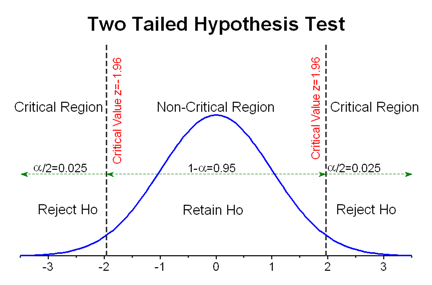
\includegraphics[scale=0.8]{twotailedtest.png}
\end{center}

\paragraph{Bonferroni-Holm-Test}
\begin{itemize}
 \item $\phi=(\phi_1,...,\phi_m)^T $ - multipler Test
 \item $\phi=(p_1,...,p_m)^T $ - zu Tests gehörende p-Werte
 \item $p_{(1)} \leq ... \leq p_{(m)} $ - geordnete p-Werte
 \item $H_{(1)},...,H_{(m)} $ - zu geordneten p-Werten gehörende Nullhypothesen
 \item $\tilde{\alpha}_j := 
	\begin{cases}
	 \frac{a}{j} & , \text{ falls } p_j(X) \text{ nicht unabhängig } \\
	 1-(1-\alpha)^{\frac{1}{j}} & , \text{ falls } p_j(X) \text{ unabhängig }
	\end{cases}
	$
 \item $\phi^{BH}=(\phi_1^{BH},...,\phi_m^{BH})^T$ mit \\
 $\phi_j^{BH} := 
      \begin{cases}
       1 & ,\text{ falls } j \leq j^* \\
       0 & ,\text{ falls } j > j^* \\
      \end{cases}
      $\\
      wobei $j^* =\max\{ \max\{j \in I_0(\theta) \cdot p_{(k)} \leq \tilde{\alpha}_{m-k+1}$ für alle $k \in \{1,...,j\}\}, 0 \}$
\end{itemize}
\paragraph{Beispiel}
\[ p_{(1)} \leq \frac{\alpha}{m} = \tilde{\alpha}_1 \]
\[ p_{(2)} \leq \frac{\alpha}{m-1} = \tilde{\alpha}_1 \]
\[ p_{(3)} \textcolor{red}{>} \frac{\alpha}{m-2} = \tilde{\alpha}_1 \]
\[ p_{(4)} > \frac{\alpha}{m-3} = \tilde{\alpha}_1 \]
\[ p_{(5)} \leq \frac{\alpha}{m-4} = \tilde{\alpha}_1 \]
$\Rightarrow \phi^{BH}$ ist multipler Test zum multiplen Niveau $\alpha$  \\
\textbf{Info:} \\
Bonferroni-Holm ist beser als Bonferroni bzw. \v Sid\'ak bzgl. Typ-II-Fehlern\\
$\rightarrow$ ''step-down''-Verfahren

\section{False Discover Rate (FDR) }
\begin{tabular}{c|c|c|c}
0-Hyp\ Test & nicht ablehnen & ablehnen & \\ \hline
wahr & \cellcolor{yellow!25} $m_0 (\theta) - V(\theta)$ & \cellcolor{yellow!25}$V(\theta)$ & \cellcolor{yellow!25}$m_0(\theta)$\\ \hline
falsch &\cellcolor{yellow!25}$m_A (\theta) - S(\theta)$  &\cellcolor{yellow!25} $S(\theta)$ &\cellcolor{yellow!25} $m_A(\theta)$\\ \hline
& \cellcolor{red!25}$m-R(\theta)$ & \cellcolor{red!25}$R(\theta)$ & m\\
\end{tabular}
\todo[inline]{yellow=unbekannt\\ red=bekannt}

\begin{itemize}
 \item $m$ - Anzahl der Tests \\
 \item $m_0 (\theta)$ - Anzahl der unter $\theta$ wahren Nullhypothesen \\
 \item $m_A (\theta)$ - Anzahl der unter $\theta$ falschen Nullhypothesen \\
 \item $R(\theta) = \sum\limits_{j=1}^m \phi_j$ - Anzahl unter $\theta$ verworfener Nullhypothesen
 \item $V(\theta) = \sum\limits_{j \in I_0(\theta)} \phi $ (zufällige) Anzahl unter $\theta$ fälschlicherweise verworfener Nullhypothese 
 \item $S(\theta) = \sum\limits_{j \in I_A(\theta)} \phi $ (zufällige) Anzahl unter $\theta$ korrekterweise verworfener Nullhypothese 
\end{itemize}

\[ \text{FDR}_{\theta}(\phi) := \text{E} \left( \frac{V(\theta}{\max\{R(\theta),1\}}\right) \]
$\rightarrow$ Multipler Test $\phi$ heißt \underline{FDR-kontrollierend zum Niveau $\alpha$}, falls
\[ \text{FDR}_{\theta}(\phi) \leq \alpha \text{ für alle } \theta \in \Theta \]

%Vorlesung vom 30.11.17

\section{Zwischenfazit Multiples Testen}
\underline{Gegeben:} 
\begin{itemize}
 \item $X=(X_1,...,X_n)^T \in S^n$
 \item $H_0$ - Nullhypothese
 \item $H_A$ - Alternativhypothese
 \item 1 Test \\ $\rightarrow$ Fehler 1.Art: $P(\phi=1,\theta \in H_0) \leq \alpha$
 \item $m > 1$ Tests $\rightarrow$ FWER=$P \left(\bigcup_{j \in I_0(\theta)} \{ \phi_j = 1 \} \right) > \alpha$
 \begin{itemize}
  \item Bonferroni
  \item \v Sid\'ak
  \item Bonferroni-Holm(``step-down''-Verfahren)
 \end{itemize}
 $\rightarrow \text{ FDR}_{\theta}(\phi) := E \frac{V(\theta)}{\max\{R(\theta),1\}}$
\end{itemize}
[Nebenbemerkung: Falls für alle $j \in  \{1,...,m\} \theta \in H_0^{(j)}, \text{dann gilt FWER}_{\theta}(\phi)=\text{FDR}_{\theta}(\phi)$ ]
\paragraph{Interpretation:}
Für $\alpha=0,05$ gilt dann $\phi$ liefert unter 100 Verwerfungen im Mittel maximal 5 fälschlicherweise verworfene Nullhypothesen
\section{Benjamin-Hochberg-Test}
\begin{itemize}
 \item $\phi=(\phi_1,...,\phi_m)^{T}$ - multipler Test 
 \item $p=(p_1,...,p_m)^{T}$ - zu Test gehörende p-Werte 
 \item $p_{(q)} \leq ... \leq p_{(m)}$ - geordnete p-Werte 
 \item $\tilde{\alpha_{j}} := j \frac{a}{m} , j \in \{1,...,m\}$ 
 \item $\phi^{FDR} = \left(\phi_{1}^{FDR},...,\phi_{m}^{FDR}\right)^{T}$ mit 
 \begin{itemize}
  \item $\phi_{1}^{FDR} = \begin{cases}
                           1, &  \text{ falls } j < j^* \\
                           0, &  \text{ falls } j \geq j^*
                          \end{cases}$ mit
 \item $j^{*}:=\min \{ \min \{j \in \{1,...,m \}: p_{(k)} > \tilde{\alpha}_{k}$ für alle $k \in \{j,...,m\} \}, m+1 \}$
 \end{itemize}
\item $P_j(X)$ unabhängig, $j \in \{1,...,m\}$
\end{itemize}

\begin{exmp}
\[ p_{(1)} \leq \tilde{\alpha}_1  = 1 \cdot \frac{\alpha}{6} \textcolor{green}{H_0 \text{ ablehnen}} \]
\[ p_{(2)} > \tilde{\alpha}_2  = 2 \cdot \frac{\alpha}{6} \textcolor{green}{H_0 \text{ ablehnen}}\]
\[ p_{(3)} \leq \tilde{\alpha}_3  = 3 \cdot \frac{\alpha}{6} \textcolor{green}{H_0 \text{ ablehnen}}\]
\[\textcolor{red}{j^*}\hspace{0.5cm} p_{(4)} > \tilde{\alpha}_4  = 4 \cdot \frac{\alpha}{6} \textcolor{green}{H_0 \text{ NICHT ablehnen}}\]
\[ p_{(5)} > \tilde{\alpha}_5  = 5 \cdot \frac{\alpha}{6} \textcolor{green}{H_0 \text{ NICHT ablehnen}}\]
\[ p_{(6)} > \tilde{\alpha}_6  = 6 \cdot \frac{\alpha}{6} \textcolor{green}{H_0 \text{ NICHT ablehnen}}\]
\end{exmp}

$\Rightarrow \phi^{FDR}$ ist FDR-kontrollierend zum Niveau $\alpha$  \\
$\Rightarrow$ ``Step-up''-Verfahren

